\documentclass[aspectratio=169]{beamer}
\usetheme{Madrid}
\usecolortheme{seahorse}
\setbeamertemplate{navigation symbols}{}
\setbeamertemplate{footline}[frame number]
\usepackage[T1]{fontenc}
\usepackage[utf8]{inputenc}
\usepackage{booktabs}
\usepackage{tikz}
\usepackage{listings}
\usetikzlibrary{arrows.meta,positioning,shapes.geometric}
\lstset{basicstyle=\ttfamily\scriptsize,breaklines=true,frame=single,
        backgroundcolor=\color{gray!10},xleftmargin=6pt,xrightmargin=6pt}

\title{ESG RAG Pipeline: Implementation and Lab}
\subtitle{What we built for the ESG RAG hands-on tutorial}
\author{Motaz K. H. Saad \and Antonella Longo}
\institute{DataLab, Dept.\ of Engineering for Innovation, University of Salento}
\date{ESG RAG tutorial --- companion code walkthrough}

\begin{document}

% 1
\begin{frame}
  \titlepage
  \vspace{-0.5em}
  \small Code: \path{esg-rag/} in the tutorial repository --- Apache-2.0
  \vfill
  \hfill
\includegraphics[height=1.5cm]{unisalento-logo.pdf}
\end{frame}

% ===== Part I: why ESG reporting exists =====
\begin{frame}
  \begin{center}
    \vspace{1.2cm}
    {\Large\bfseries Part I --- Why ESG disclosure exists}\\[4mm]
    {\large From mandatory reporting to decision-grade data}\\[8mm]
    \small Financial reports tell one story. Sustainability reports tell another.
  \end{center}
\end{frame}

\begin{frame}{One company, two accountability channels}
  \footnotesize
  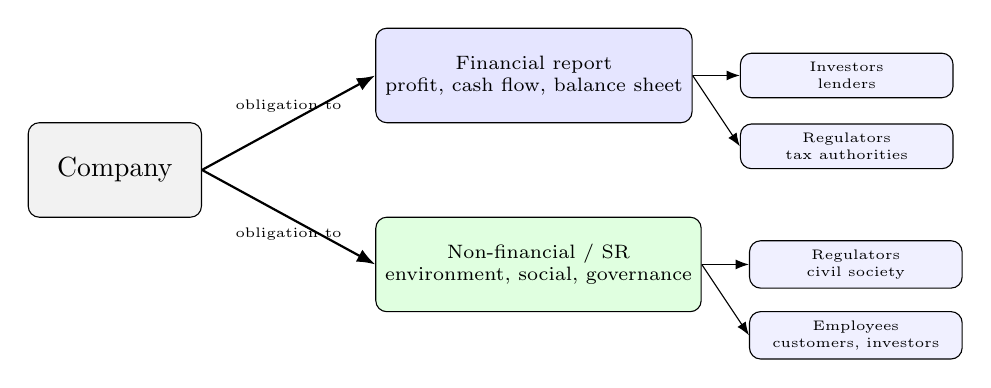
\begin{tikzpicture}[>=Latex, node distance=3mm,
      co/.style={draw,fill=gray!10,rounded corners,align=center,minimum width=22mm,minimum height=12mm},
      rp/.style={draw,rounded corners,align=center,minimum width=40mm,minimum height=12mm,font=\scriptsize},
      au/.style={draw,fill=blue!6,rounded corners,align=center,minimum width=27mm,font=\tiny}]
    \node[co] (c) {Company};
    \node[rp,fill=blue!10,right=22mm of c,yshift=12mm] (fin) {Financial report\\profit, cash flow, balance sheet};
    \node[rp,fill=green!12,right=22mm of c,yshift=-12mm] (sus) {Non-financial / SR\\environment, social, governance};
    \draw[->,thick] (c.east) -- node[above,font=\tiny]{obligation to} (fin.west);
    \draw[->,thick] (c.east) -- node[below,font=\tiny]{obligation to} (sus.west);
    \node[au,right=6mm of fin] (i1) {Investors\\lenders};
    \node[au,right=6mm of fin,yshift=-9mm] (i2) {Regulators\\tax authorities};
    \node[au,right=6mm of sus] (s1) {Regulators\\civil society};
    \node[au,right=6mm of sus,yshift=-9mm] (s2) {Employees\\customers, investors};
    \draw[->] (fin.east) -- (i1.west); \draw[->] (fin.east) -- (i2.west);
    \draw[->] (sus.east) -- (s1.west); \draw[->] (sus.east) -- (s2.west);
  \end{tikzpicture}
  \vspace{2mm}
  \begin{itemize}
    \item \textbf{Financial reporting}: economic performance, standardized accounting, primarily for capital providers.
    \item \textbf{Sustainability reporting}: impacts, risks and opportunities beyond the income statement --- and increasingly \emph{also} for investors.
  \end{itemize}
\end{frame}

\begin{frame}{Why non-financial reporting became mandatory}
  \footnotesize
  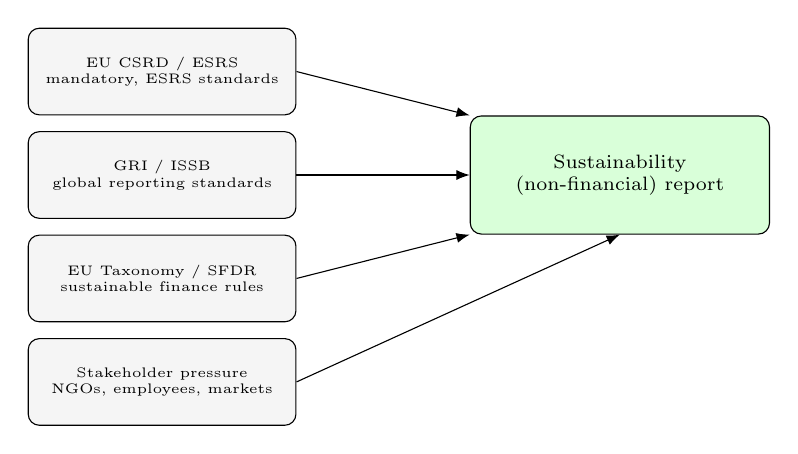
\begin{tikzpicture}[>=Latex, node distance=2mm,
      drv/.style={draw,fill=gray!8,rounded corners,align=center,minimum width=34mm,minimum height=11mm,font=\tiny},
      core/.style={draw,fill=green!15,rounded corners,align=center,minimum width=38mm,minimum height=15mm,font=\scriptsize}]
    \node[drv] (a) {EU CSRD / ESRS\\mandatory, ESRS standards};
    \node[drv,below=of a] (b) {GRI / ISSB\\global reporting standards};
    \node[drv,below=of b] (c) {EU Taxonomy / SFDR\\sustainable finance rules};
    \node[drv,below=of c] (d) {Stakeholder pressure\\NGOs, employees, markets};
    \node[core,right=22mm of b] (e) {Sustainability\\(non-financial) report};
    \draw[->] (a.east) -- (e.north west);
    \draw[->] (b.east) -- (e.west);
    \draw[->] (c.east) -- (e.south west);
    \draw[->] (d.east) -- (e.south);
  \end{tikzpicture}
  \vspace{1mm}
  \begin{itemize}
    \item \textbf{Double materiality}: report both the company's impact on people/planet \emph{and} how ESG issues affect the company.
    \item Regulated, comparable, audited data --- but delivered as \textbf{text, tables and PDFs}, not a database.
  \end{itemize}
\end{frame}

\begin{frame}{What is inside a sustainability report?}
  \begin{columns}[T]
    \begin{column}{0.31\textwidth}
      \begin{block}{E --- Environmental}
        \scriptsize
        GHG Scope 1/2/3 emissions\\
        Energy, renewables\\
        Water, waste, materials\\
        Biodiversity, EU Taxonomy alignment
      \end{block}
    \end{column}
    \begin{column}{0.31\textwidth}
      \begin{block}{S --- Social}
        \scriptsize
        Employees, hires, turnover\\
        Training hours\\
        Diversity, gender pay gap\\
        Health \& safety, human rights
      \end{block}
    \end{column}
    \begin{column}{0.31\textwidth}
      \begin{block}{G --- Governance}
        \scriptsize
        Board composition\\
        Committees, independence\\
        Anti-corruption, tax strategy\\
        Executive pay, risk management
      \end{block}
    \end{column}
  \end{columns}
  \vspace{2mm}
  \begin{itemize}
    \item KPIs are referenced to standards (e.g.\ \texttt{GRI 305-1}, \texttt{GRI 2-7}) and appear as \textbf{narratives and tables}.
    \item The same KPI may be reported in different units, years, languages (EN/IT) and report sections.
  \end{itemize}
\end{frame}

\begin{frame}{Double materiality: why investors care too}
  \footnotesize
  \begin{center}
  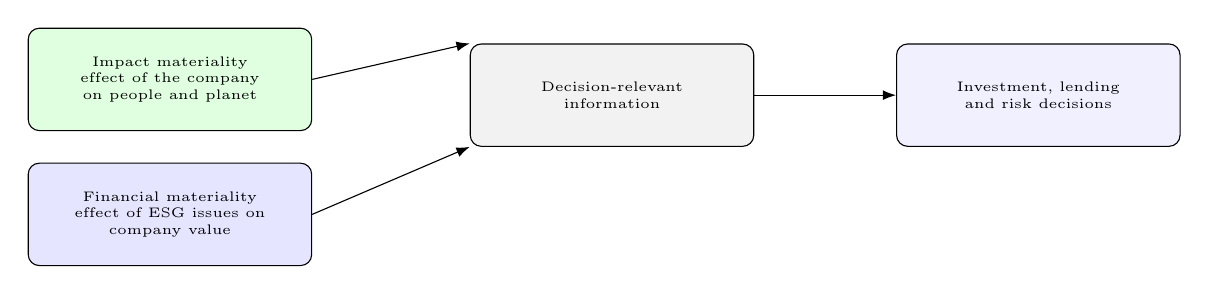
\begin{tikzpicture}[>=Latex, node distance=2mm,
      box/.style={draw,rounded corners,align=center,minimum width=36mm,minimum height=13mm,font=\tiny}]
    \node[box,fill=green!12] (impact) {Impact materiality\\effect of the company\\on people and planet};
    \node[box,fill=blue!10,below=4mm of impact] (finm) {Financial materiality\\effect of ESG issues on\\company value};
    \node[box,fill=gray!10,right=20mm of impact,yshift=-2mm] (mat) {Decision-relevant\\information};
    \node[box,fill=blue!6,right=18mm of mat] (use) {Investment, lending\\and risk decisions};
    \draw[->] (impact.east) -- (mat.north west);
    \draw[->] (finm.east) -- (mat.south west);
    \draw[->] (mat.east) -- (use.west);
  \end{tikzpicture}
  \end{center}
  \vspace{1mm}
  \begin{itemize}
    \item Climate \textbf{transition risk} and \textbf{physical risk}, carbon pricing, regulation and fines.
    \item Reputation, talent, supply-chain resilience and access to capital.
    \item Investors therefore need the \emph{same} disclosed numbers that regulators audit --- but at portfolio scale.
  \end{itemize}
\end{frame}

\begin{frame}{From disclosure to decision}
  \footnotesize
  \begin{center}
  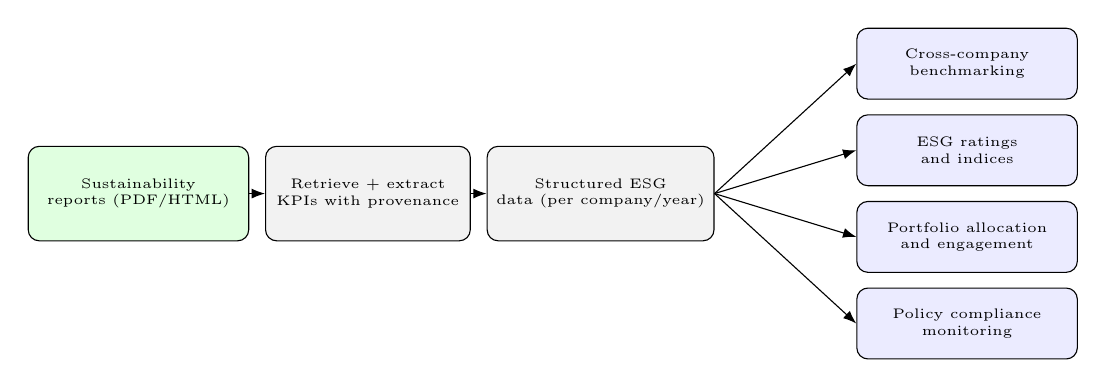
\begin{tikzpicture}[>=Latex, node distance=2mm,
      st/.style={draw,fill=green!12,rounded corners,align=center,minimum width=28mm,minimum height=12mm,font=\tiny},
      mid/.style={draw,fill=gray!10,rounded corners,align=center,minimum width=26mm,minimum height=12mm,font=\tiny},
      endd/.style={draw,fill=blue!8,rounded corners,align=center,minimum width=28mm,minimum height=9mm,font=\tiny}]
    \node[st] (rep) {Sustainability\\reports (PDF/HTML)};
    \node[mid,right=of rep] (pipe) {Retrieve + extract\\KPIs with provenance};
    \node[mid,right=of pipe] (data) {Structured ESG\\data (per company/year)};
    \node[endd,right=18mm of data,yshift=16.5mm] (u1) {Cross-company\\benchmarking};
    \node[endd,right=18mm of data,yshift=5.5mm] (u2) {ESG ratings\\and indices};
    \node[endd,right=18mm of data,yshift=-5.5mm] (u3) {Portfolio allocation\\and engagement};
    \node[endd,right=18mm of data,yshift=-16.5mm] (u4) {Policy compliance\\monitoring};
    \draw[->] (rep)--(pipe); \draw[->] (pipe)--(data);
    \foreach \y in {u1,u2,u3,u4} \draw[->] (data.east) -- (\y.west);
  \end{tikzpicture}
  \end{center}
  \vspace{1mm}
  \small The bottleneck is turning heterogeneous documents into \textbf{verifiable, comparable data}.
\end{frame}

\begin{frame}{Who uses ESG data, and for what?}
  \small
  \begin{table}
    \centering
    \begin{tabular}{p{0.26\textwidth}p{0.30\textwidth}p{0.38\textwidth}}
    \toprule
    Actor & Typical question & Use of the data \\
    \midrule
    Investors & Is the company exposed to transition risk? & Allocation, valuation, engagement, stewardship \\
    Policy makers / regulators & Are CSRD/ESRS disclosures complete and consistent? & Compliance monitoring, regulation design \\
    Companies & How do we compare with peers and targets? & Strategy, target setting, supplier screening \\
    Lenders / insurers & What is the ESG risk in this portfolio? & Pricing, due diligence, risk provisions \\
    Researchers / NGOs & Are the public claims verifiable? & Accountability, empirical studies \\
    \bottomrule
    \end{tabular}
  \end{table}
  \vspace{2mm}
  \begin{itemize}
    \item All of them need \textbf{evidence}: which report, which passage, which year, which unit.
  \end{itemize}
\end{frame}

\begin{frame}{From a report to an auditable answer}
  \small
  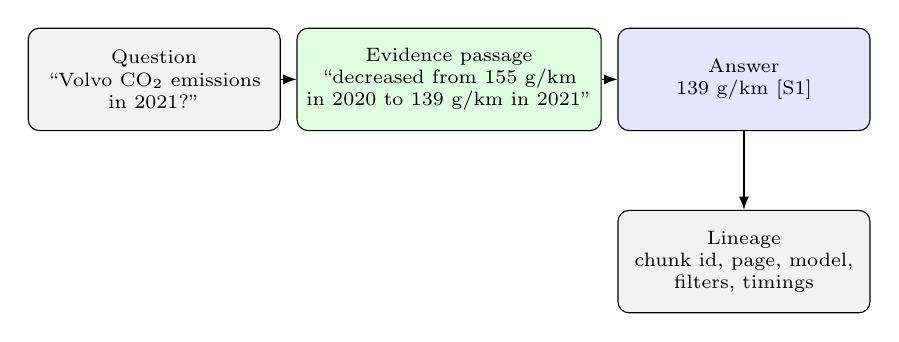
\begin{tikzpicture}[>=Latex, node distance=2mm,
      bx/.style={draw,rounded corners,align=center,minimum width=32mm,minimum height=13mm,font=\scriptsize}]
    \node[bx,fill=gray!10] (q) {Question\\``Volvo CO$_2$ emissions\\in 2021?''};
    \node[bx,fill=green!12,right=of q] (p) {Evidence passage\\``decreased from 155 g/km\\in 2020 to 139 g/km in 2021''};
    \node[bx,fill=blue!10,right=of p] (a) {Answer\\139 g/km [S1]};
    \node[bx,fill=gray!10,below=10mm of a] (l) {Lineage\\chunk id, page, model,\\
      filters, timings};
    \draw[->] (q)--(p); \draw[->] (p)--(a); \draw[->] (a.south)--(l.north);
  \end{tikzpicture}
  \vspace{2mm}
  \begin{itemize}
    \item This is the running example in the lab --- and exactly what the pipeline automates.
    \item The citation \texttt{[S1]} is a pointer to stored evidence, not a decorative footnote.
  \end{itemize}
\end{frame}

\begin{frame}
  \begin{center}
    \vspace{1.2cm}
    {\Large\bfseries Part II --- What we implemented}\\[4mm]
    {\large A working, local-first ESG RAG pipeline}\\[8mm]
    \small Data $\to$ index $\to$ retrieval techniques $\to$ answers $\to$ evidence $\to$ dashboard
  \end{center}
\end{frame}

% 2
\begin{frame}{What was built}
  \begin{columns}[T]
    \begin{column}{0.55\textwidth}
      \begin{itemize}
        \item A \textbf{working, local-first} ESG RAG pipeline --- no API keys, no cloud.
        \item Two local Ollama models in the smoke test:
          \begin{itemize}
            \item \texttt{qwen3:4b-instruct} (generator / judge)
            \item \texttt{embeddinggemma:latest} (embedder)
          \end{itemize}
        \item Real published ESG data sampled from the presenters' companion repos.
        \item \textbf{Everything parameterised}: models, chunking, retrieval, generation, evaluation.
        \item \textbf{7 RAG techniques}, a \textbf{2$\times$2 model matrix}, a \textbf{web dashboard}.
        \item Machine-readable results: JSON / CSV / Markdown / JSONL lineage.
      \end{itemize}
    \end{column}
    \begin{column}{0.43\textwidth}
      \footnotesize
      \path{esg-rag/}\\
      \quad \path{esg_rag/}\\
      \quad\quad config.py, ollama.py\\
      \quad\quad chunking.py, indexing.py\\
      \quad\quad retrieval.py, strategies.py\\
      \quad\quad generation.py, extraction.py\\
      \quad\quad evaluate.py, lineage.py\\
      \quad\quad pipeline.py, cli.py\\
      \quad \path{data/}, \path{docs/}, \path{dashboard/}\\
      \quad \path{output/results/}
    \end{column}
  \end{columns}
\end{frame}

% 3
\begin{frame}{End-to-end pipeline}
  \footnotesize
  \begin{tikzpicture}[node distance=2mm, >=Latex,
      box/.style={draw,rounded corners,fill=blue!8,align=center,minimum height=9mm,font=\scriptsize},
      lbl/.style={font=\tiny,text=gray!70!black}]
    \node[box] (a) {Parse\\corpus};
    \node[box,right=of a] (b) {Chunk\\(3 strategies)};
    \node[box,right=of b] (c) {Embed\\(2 models)};
    \node[box,right=of c] (d) {Vector index\\+ metadata};
    \node[box,below=7mm of d] (e) {Retrieve\\(dense/BM25/hybrid)};
    \node[box,left=of e] (f) {Generate / extract\\(7 techniques)};
    \node[box,left=of f] (g) {Answer + citations\\or KPI JSON};
    \node[box,below=7mm of g] (h) {Lineage + metrics};
    \draw[->] (a)--(b); \draw[->] (b)--(c); \draw[->] (c)--(d);
    \draw[->] (d)--(e); \draw[->] (e)--(f); \draw[->] (f)--(g); \draw[->] (g)--(h);
    \node[lbl,below=1mm of a] {\path{chunking.py}};
    \node[lbl,below=1mm of c] {\path{ollama.py}};
    \node[lbl,below=1mm of e] {\path{retrieval.py}};
    \node[lbl,below=1mm of g] {\path{generation.py}};
    \node[lbl,below=1mm of h] {\path{lineage.py}};
  \end{tikzpicture}
  \vspace{2mm}
  \begin{itemize}
    \item One \texttt{ESGRAGPipeline} object is shared by the CLI, REST service, smoke test, matrix runner and dashboard.
    \item Each query writes an append-only record: question, filters, config, source chunks, answer, trace, timings.
  \end{itemize}
\end{frame}

% 4
\begin{frame}{Two corpora: smoke test and published real data}
  \small
  \begin{table}
    \centering
    \begin{tabular}{p{0.24\textwidth}p{0.36\textwidth}p{0.34\textwidth}}
    \toprule
     & Synthetic smoke corpus & Real published sample \\
    \midrule
    Source & Fictional reports written for the lab & \path{ESG-RAG-benchmark-ragas} (IEEE BigData 2026, MIT) \\
    Size & 2 reports $\to$ 8 chunks (EN + IT) & 6 verbatim report excerpts ($\sim$2.5--3 KB) \\
    Questions & \path{gold.jsonl}: 3 literal answers & \path{real_qa.json}: 6 QA pairs + ESG pillar \\
    IR benchmark & --- & \path{real_retrieval_bench.json}: 24 graded queries \\
    License & lab code & \path{benchmark-embeddings-esg} (ITADATA 2026, Apache-2.0) \\
    \bottomrule
    \end{tabular}
  \end{table}
  \begin{itemize}
    \item Real excerpts keep upstream wording, \texttt{*Page N*} markers, and a metadata header with full source URL.
    \item \path{data/PROVENANCE.md} records exact upstream paths and sampling method.
  \end{itemize}
\end{frame}

% 5
\begin{frame}[fragile]{Chunking and metadata are parameters}
  \begin{columns}[T]
    \begin{column}{0.52\textwidth}
      \begin{itemize}
        \item \textbf{section} (default): headings delimit chunks; GRI codes and pages are kept as metadata.
        \item \textbf{fixed}: plain overlapping word windows.
        \item \textbf{semantic}: adjacent paragraphs grouped by vocabulary overlap.
        \item Knobs: \texttt{max\_words}, \texttt{overlap\_words}, \texttt{min\_words}, \texttt{semantic\_threshold}.
      \end{itemize}
    \end{column}
    \begin{column}{0.46\textwidth}
      \scriptsize
      Metadata attached to every chunk:\\
      \texttt{company}, \texttt{report\_year}, \texttt{language},\\
      \texttt{country}, \texttt{section}, \texttt{gri\_reference},\\
      \texttt{pdf/source file}, \texttt{page}, \texttt{source\_url},\\
      \texttt{license}, \texttt{source\_repo}.\\
      \vspace{2mm}
      Used for filtered retrieval, citations and lineage.
    \end{column}
  \end{columns}
  \vspace{2mm}
  \begin{lstlisting}
python3 -m esg_rag.cli --set chunking.strategy=semantic \
  --set chunking.semantic_threshold=0.2 index --corpus real
  \end{lstlisting}
\end{frame}

% 6
\begin{frame}{Embeddings and the vector index}
  \begin{itemize}
    \item \textbf{Two embedders}, both served by Ollama:
      \begin{itemize}
        \item \texttt{embeddinggemma:latest} --- 768 dimensions
        \item \texttt{qwen3-embedding:0.6b} --- 1024 dimensions (pulled for the matrix)
      \end{itemize}
    \item One index per \textbf{corpus $\times$ embedder}, persisted as JSON.
    \item Exact L2-normalised cosine similarity in pure Python (optional NumPy); no FAISS/Chroma download needed.
    \item Metadata pre-filtering before search; index fingerprint stored in every lineage record.
    \item \texttt{VectorStore} is the only storage-aware component --- swap for FAISS / Milvus / DiskANN without touching retrieval or generation.
  \end{itemize}
  \vspace{1mm}
  \small \texttt{index\_real\_embeddinggemma\_latest.json}, \texttt{index\_real\_qwen3-embedding\_0\_6b.json}
\end{frame}

% 7
\begin{frame}{Retrieval: dense, lexical and hybrid}
  \begin{columns}[T]
    \begin{column}{0.52\textwidth}
      \begin{itemize}
        \item \textbf{dense}: cosine similarity over query embedding.
        \item \textbf{BM25}: Okapi scoring over the chunk text; pure Python.
        \item \textbf{hybrid} (default): reciprocal rank fusion of both candidate lists.
      \end{itemize}
      \scriptsize
      $\mathrm{RRF}(d)=\sum_{lists}\frac{1}{k+\mathrm{rank}_{list}(d)}$
    \end{column}
    \begin{column}{0.46\textwidth}
      \scriptsize
      \textbf{Why lexical matters:}\\
      GRI codes, KPI names and units (\texttt{tCO2e}, \texttt{g/km}) are rare literal tokens.\\
      \vspace{2mm}
      \textbf{Filters:}\\
      \texttt{--company}, \texttt{--year}, \texttt{--gri}, \texttt{--section}, or \texttt{--filter key=value}.\\
      String filters support substring and \texttt{prefix*} matching.\\
      Optional LLM-inferred filters (\texttt{retrieval.infer\_filters}).
    \end{column}
  \end{columns}
\end{frame}

% 8
\begin{frame}{Seven RAG techniques (one contract)}
  \small
  \begin{table}
    \centering
    \begin{tabular}{p{0.22\textwidth}p{0.44\textwidth}p{0.28\textwidth}}
    \toprule
    Technique & What it does & Extra LLM calls \\
    \midrule
    \texttt{naive} & dense top-k $\to$ generate & 0 \\
    \texttt{hybrid} & dense + BM25 $\to$ RRF $\to$ generate & 0 \\
    \texttt{filtered} & hybrid + metadata predicates (optionally inferred) & 0--1 \\
    \texttt{multi\_query} & rewrite into N queries, retrieve each, fuse ranks & 1 \\
    \texttt{rerank} & retrieve large pool, LLM scores passages 0--5 & 1 \\
    \texttt{self\_rag} & grade evidence; rewrite + retry if unsupported & 1--2 \\
    \texttt{decompose} & split question, answer sub-questions, synthesize & $2+$ \\
    \bottomrule
    \end{tabular}
  \end{table}
  \begin{itemize}
    \item Same output contract for all: answer, citations, evidence, \texttt{trace}, latency, tokens.
    \item Each internal step is recorded in the lineage log and shown in the dashboard.
  \end{itemize}
\end{frame}

% 9
\begin{frame}{Grounded generation and faithfulness}
  \begin{columns}[T]
    \begin{column}{0.54\textwidth}
      \begin{itemize}
        \item The generator sees \textbf{only} retrieved passages, never the raw corpus.
        \item Rules in the system prompt:
          \begin{enumerate}
            \item use only evidence;
            \item cite every claim as \texttt{[S1]}, \texttt{[S2]};
            \item at most two short sentences;
            \item never invent numbers or units;
            \item say \texttt{INSUFFICIENT EVIDENCE} if unsupported.
          \end{enumerate}
        \item Optional LLM judge returns \texttt{\{supported, explanation\}} in JSON mode.
      \end{itemize}
    \end{column}
    \begin{column}{0.44\textwidth}
      \scriptsize
      \textbf{Example output (real data)}\\[1mm]
      ``The average CO$_2$ emissions of Volvo cars sold in Europe in 2021 were 139 g/km [S1].''\\[2mm]
      Evidence: \texttt{377\_60\_2021::c002}, company Volvo Cars, year 2021, page marker preserved.
    \end{column}
  \end{columns}
\end{frame}

% 10
\begin{frame}[fragile]{Document $\to$ structured data: KPI extraction}
  \begin{itemize}
    \item KPI prompts mirror the SESG case study: \path{prompts.yaml} with \textbf{59 GRI questions}; 5 bundled in the lab.
    \item Each question carries its expected JSON schema and target table (\texttt{kpi\_emissions}, \texttt{kpi\_employee}, \ldots).
    \item Ollama \texttt{format: json} constrains the output; the parsed object is attached to passages and timings.
  \end{itemize}
  \vspace{1mm}
  \begin{lstlisting}
python3 -m esg_rag.cli extract "GRI 305_305-1_32" --company Nordwind

{"reporting year": "2023", "value": 84320, "unit": "tCO2e"}
  \end{lstlisting}
  \small Provenance: target table \texttt{kpi\_emissions} + source chunk id + metadata.
\end{frame}

% 11
\begin{frame}{Everything is parameterised}
  \small
  \begin{table}
    \centering
    \begin{tabular}{p{0.25\textwidth}p{0.69\textwidth}}
    \toprule
    Config section & Controls \\
    \midrule
    \texttt{models} & generator, embedder, judge, rewrite, rerank, model pools \\
    \texttt{chunking} & strategy, max/overlap/min words, semantic threshold \\
    \texttt{retrieval} & mode, top-k, BM25 $k_1/b$, RRF $k$, evidence length, filters \\
    \texttt{strategy} & active technique, rewrite count, rerank depth, self-RAG loops \\
    \texttt{generation} & temperature, max tokens, seed, context, thinking \\
    \texttt{benchmark}, \texttt{matrix} & dataset, limit, judge, model pools, techniques \\
    \texttt{system\_metrics} & telemetry on/off, power source, fallback watts \\
    \bottomrule
    \end{tabular}
  \end{table}
  \begin{itemize}
    \item Three ways to override: \path{config.yaml}, \texttt{ESG\_RAG\_*} env vars, and \texttt{--set section.key=value} (repeatable).
  \end{itemize}
\end{frame}

% 12
\begin{frame}{Systems metrics reported next to quality}
  \small
  \begin{tabular}{p{0.32\textwidth}p{0.40\textwidth}p{0.22\textwidth}}
  \toprule
  Metric & Source & Meaning \\
  \midrule
  \texttt{tokens\_per\_second} & Ollama \texttt{eval\_duration} / \texttt{eval\_count} & decode speed \\
  \texttt{memory} & \texttt{/proc/self/statm}, Ollama \texttt{/api/ps} & process RSS, model size, VRAM \\
  \texttt{energy\_j}, \texttt{avg\_watts} & RAPL / NVIDIA-SMI if readable; else estimate & joules and power per query \\
  \texttt{latency}, \texttt{tokens}, \texttt{llm\_calls} & pipeline timers & cost and complexity \\
  \bottomrule
  \end{tabular}
  \vspace{2mm}
  \begin{itemize}
    \item On this CPU-only laptop: \textbf{6--8 tok/s}, \textbf{38--39 MB} lab RSS, \textbf{3.9--4.4 GB} loaded models in RAM.
    \item RAPL is root-only and there is no GPU, so energy is an \textbf{explicitly labelled estimate}: \texttt{power\_measured = false}.
    \item Never present estimated joules as a measurement --- the flag makes this auditable.
  \end{itemize}
\end{frame}

% 13
\begin{frame}{Benchmark harness and real results}
  \small
  \begin{itemize}
    \item Matrix: \textbf{2 LLMs} (qwen3, gemma3) $\times$ \textbf{2 embedders} (embeddinggemma, qwen3-embedding) $\times$ \textbf{5 techniques} $\times$ 2 real questions = \textbf{20 cells}.
    \item Retrieval-only benchmark: 24 graded ESG query/document triples: NDCG@10 $\approx$ \textbf{0.97} for both embedders, MRR/P@1 = 1.0.
  \end{itemize}
  \vspace{1mm}
  \begin{table}
    \centering
    \footnotesize
    \begin{tabular}{p{0.34\textwidth}p{0.18\textwidth}p{0.18\textwidth}p{0.20\textwidth}}
    \toprule
    Observation & qwen3:4b-instruct & gemma3:4b & Advanced techniques \\
    \midrule
    Answer hit rate & 1.00 in all techniques & 0.50 with \texttt{rerank} & no gain on this sample \\
    Avg latency & \multicolumn{2}{c}{naive 66.7 s, hybrid 60.0 s} & rerank 132.4 s \\
    Judge support & \multicolumn{2}{c}{most cells 1.0} & \texttt{self\_rag} 0.5 \\
    \bottomrule
    \end{tabular}
  \end{table}
  \vspace{1mm}
  \scriptsize Caveat: 2 questions on a CPU laptop --- a demonstration of the methodology, not a paper-quality comparison.
\end{frame}

% 14
\begin{frame}{Results are artefacts, not screenshots}
  \small
  \begin{table}
    \centering
    \begin{tabular}{p{0.40\textwidth}p{0.54\textwidth}}
    \toprule
    Artefact & Contents \\
    \midrule
    \path{matrix.json} & full config, 20 cell summaries, per-question answers, IR metrics \\
    \path{matrix.csv} & one row per (LLM, embedder, technique) cell \\
    \path{matrix\_report.md} & generated Markdown tables \\
    \path{matrix\_telemetry.*} & 4-cell addendum with memory / tok/s / energy columns \\
    \path{lineage.jsonl} & one append-only record per query (local-only, gitignored) \\
    \bottomrule
    \end{tabular}
  \end{table}
  \begin{itemize}
    \item Files are rewritten after \textbf{every completed cell}, so partial results are visible during long runs.
    \item The summary artefacts are versioned in git; indexes and lineage stay local.
    \item \path{docs/REAL_DATA_RESULTS.md} documents data provenance, methods and findings.
  \end{itemize}
\end{frame}

% 15
\begin{frame}{Web dashboard: observe and run experiments}
  \begin{columns}[T]
    \begin{column}{0.53\textwidth}
      \textbf{Results tab}
      \begin{itemize}
        \item auto-refresh every 8 s; LIVE progress from lineage before \path{matrix.json} exists;
        \item cards, sortable table with per-question drill-down;
        \item filters: technique, LLM, \textbf{embedder}, \textbf{ESG pillar}, question search \texttt{q};
        \item embedding-quality bars; quality-vs-X scatter with labelled x-axis and selector (latency / tok/s / energy / watts).
      \end{itemize}
    \end{column}
    \begin{column}{0.45\textwidth}
      \textbf{Configure \& Run tab}
      \begin{itemize}
        \item checkbox groups for LLMs, embedders and techniques --- combine any subset;
        \item all pipeline knobs exposed in the form;
        \item allowlisted + clamped parameters, one background job at a time;
        \item \texttt{/api/config}, \texttt{POST /api/run}, \texttt{/api/run/status}.
      \end{itemize}
    \end{column}
  \end{columns}
  \vspace{1mm}
  \small Runs at \texttt{http://127.0.0.1:8080}; no web framework or CDN required.
\end{frame}

% 16
\begin{frame}[fragile]{Reproduce it in a few commands}
  \begin{lstlisting}
cd esg-rag
python3 -m pip install -r requirements.txt
ollama pull qwen3:4b-instruct gemma3:4b embeddinggemma:latest qwen3-embedding:0.6b

./run_smoke_test.sh                       # synthetic corpus, ~1 min
python3 -m esg_rag.cli --corpus real evaluate --dataset real --strategy hybrid --limit 6
python3 -m esg_rag.cli matrix --dataset real --limit 2 --judge
python3 dashboard.py --port 8080          # http://127.0.0.1:8080
  \end{lstlisting}
  \small Or use the dashboard's Configure \& Run tab: tick models / embedders / techniques and press \textbf{Run experiment}.
\end{frame}

% 17
\begin{frame}{Takeaways for a data-management audience}
  \begin{enumerate}
    \item RAG over regulated documents is a \textbf{data pipeline problem}: parsing, chunking, metadata, indexing, provenance.
    \item \textbf{Filtered hybrid retrieval} and metadata predicates are first-class design choices, not afterthoughts.
    \item \textbf{Lineage} makes answers auditable: passages, config, models, prompts, timings in one queryable log.
    \item Report \textbf{systems metrics} (latency, memory, tok/s, energy) alongside answer quality.
    \item \textbf{Reproducible artefacts} --- JSON/CSV tables and a live dashboard --- make comparisons inspectable.
    \item Caveats to discuss: LLM-judge bias, small test sets, estimated energy, and the limits of a pure-Python vector store at corpus scale.
  \end{enumerate}
  \vspace{2mm}
  \centering \large Questions?
\end{frame}

\end{document}
